% !TEX root = ../main.tex
\subsection{Deep Inelastic Scattering}
\label{10.10::deep_inelastic_scattering}
    In its simplest description, DIS refers to the scattering of an electron off a quark inside a nucleon.
    Figure \ref{fig::10.10::dis_diagram} displays the Feynman diagram illustrating DIS.
    The four-momentum of the nucleon is denoted by $P$, while that of the quark is represented by $p$.
    The initial and final four-momenta of the electron are given by $k$ and $k'$, respectively.
    When $k'$ is measured, the momentum transferred to the hadron system by the virtual photon is defined as $q = k - k'$.
    $q$ is a spacelike vector conventionally denoted as $q^2 = -Q^2$.

    \begin{figure}[h!]
        \centering\frame{
        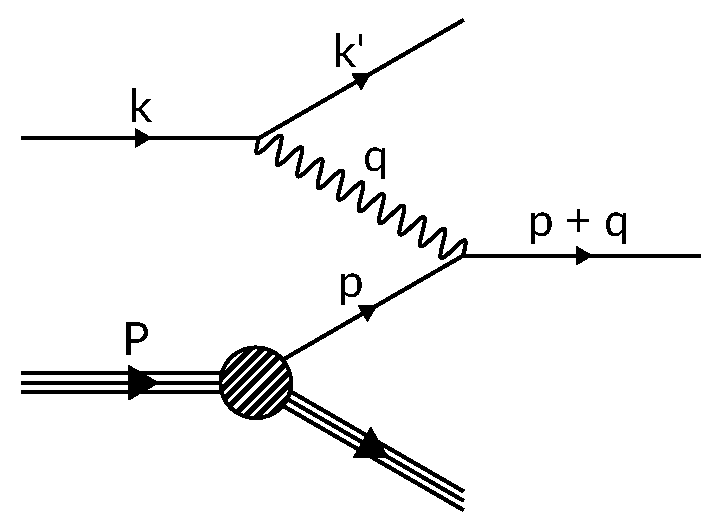
\includegraphics[width=0.6\textwidth]{10dis_diagram.pdf}}
        \caption[DIS in QCD.]{DIS in QCD. The diagram describes the stream of momentum in the scattering of a high energy electron off a quark. The quark's wave function is incorporated in the nucleon's wave function. Source: Own elaboration, using \href{https://inkscape.org/}{Inkscape}.}
        \label{fig::10.10::dis_diagram}
    \end{figure}

    If $Q^2$ is sufficiently high, the quark is ejected from the nucleon.
    Soft processes, such as gluon emission and quark-antiquark pair production, then take place to neutralise the colour charge.
    This results in the transformation of the ejected quark into a jet of hadrons.
    The jet propagates in the direction of the transferred momentum from the electron.

    % !TEX root = ../main.tex
% --+ Approximating the cross section +-----------------------------------------
To approximate the cross section of electron-nucleon scattering, we will work in the center of mass reference frame.
In this frame, the electron and nucleon are moving towards each other with sufficient energy, allowing us to neglect the nucleon's mass.
As a result, the nucleon possesses nearly lightlike momentum along the collision axis.
Consequently, the constituent quarks of the nucleon also have nearly lightlike momenta that are nearly collinear to the nucleon's momentum.
Hence, as a first-order approximation, we can express the quark's momentum as
\begin{equation*}
    p = \xi P,
\end{equation*}
where $\xi$ represents the longitudinal fraction of the quark's momentum, and thus $0 < \xi < 1$.

In the leading-order approximation, we can also disregard gluon emission and exchange during the collision.
Therefore, the cross section of electron-nucleon scattering is equal to that of electron-quark scattering for a given $\xi$, multiplied by the probability that the nucleon contains a quark with a longitudinal momentum fraction of $\xi$, integrated over $\xi$.

This calculation encounters the issue that the probability of a nucleon containing a quark with a specific momentum cannot be computed within perturbative QCD.
It relies on the soft processes that determine the nucleon's structure as a composite system of quarks and gluons.
Consequently, we must consider this probability as an unknown function that needs to be measured in experiments.

Such probability functions are known as Parton Distribution Functions (PDFs).
A PDF can be assigned to various types of quarks, antiquarks, and gluons, and is incorporated into the nucleon's wave function.
For each parton $f$, its PDF is defined as
\begin{equation*}
    P_f = f_f(\xi)d\xi.
\end{equation*}
Therefore, the cross section for the inelastic scattering of an electron off a nucleon, within the leading-order approximation, can be expressed as
\begin{equation*}
    \sigma\left( e^-(k) p(P) \rightarrow e^-(k') X \right) =
            \int_0^1d\xi \sum_f f_f(\xi) \cdot
            \sigma\left( e^-(k) q_f(\xi P) \rightarrow e^-(k') + q_f(p') \right),
\end{equation*}
where $X$ denotes the final hadronic state.
It is important to remember that this equation does not provide an exact QCD prediction but represents the first-term expansion of $\alpha_s$.
This approximation is known as the parton model \cite{halzen1991}.

    % !TEX root = ../main.tex
\subsubsection{The Parton Model}
\label{sssec::parton_model}
    \begin{figure}[b!]
        \centering
        \frame{
        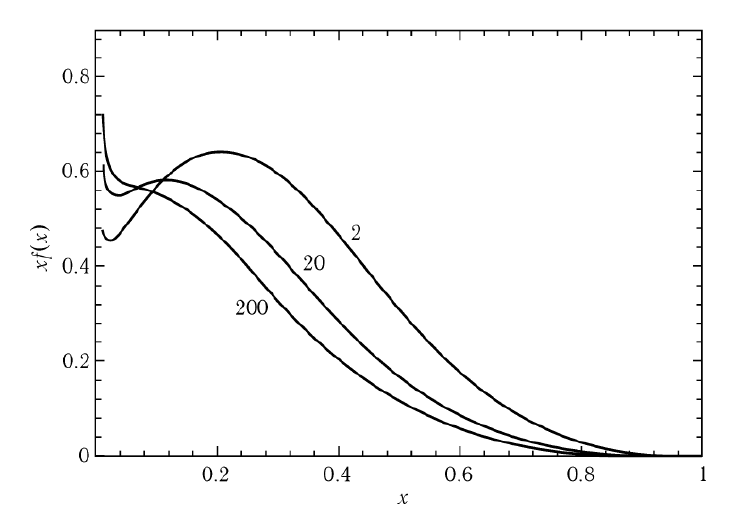
\includegraphics[width=0.8\textwidth]{12q2_dependence_u.png}}
        \caption[$Q^2$ dependence of $x$ PDF for the $u$ quark.]{Parton distribution functions $xf_f(x)$ for the $u$ quark at $Q = 2$, $Q = 20$, and $Q = 200$ GeV, showing the parton evolution effect according to the Altarelli-Parisi equations.} % NOTE. Can't find a source :(.
        \label{fig::q2dependenceu}
    \end{figure}

    In the parton model, the cross section is given by
    \begin{equation}
        \label{eq::parton_model_cross_section}
        \frac{d^2\sigma}{dxdy} \left( e^-p \rightarrow e^-X \right) =
                \left( \sum_f xf_f \left( x, Q^2 \right) Q_f^2 \right)
                \frac{2\pi\alpha s}{Q^4} \left( 1 + \left( 1 - y \right)^2 \right),
    \end{equation}
    where $s \equiv 2P\cdot k$, $Q_f$ represents the charge of parton $f$, and $x$ and $y$ are the Bjorken variables defined as
    \begin{equation*}
        x \equiv \frac{Q^2}{2P\cdot q}, \hspace{36pt} y \equiv \frac{2 P\cdot q}{s}.
    \end{equation*}
    In the nucleon's rest frame, $y = q^0/k^0$, and it represents the energy transferred to the hadron by the incoming electron.

    The PDFs in equation \eqref{eq::parton_model_cross_section} have a weak dependence on $Q^2$ due to gluon radiation.
    This leads to Bjorken scaling violation \cite{halzen1991}.
    When the structure functions are known for certain values of $Q^2$, they can be evolved to other values using the Dokshitzer-Gribov-Lipatov-Altarelli-Parisi (DGLAP) equations \cite{dokshitzer1991}.

    Figure \ref{fig::q2dependenceu} shows the predictions of the Altarelli-Parisi equations for the evolution of the PDFs with respect to $Q^2$.
    Partons with large $x$ tend to radiate and move towards states with lower $x$ values.
    Simultaneously, radiation generates new partons with low $x$ values.
    As $Q^2$ increases, the parton distributions decrease for large $x$ values while rapidly increasing for low $x$.
    At low $Q^2$, the wavelength of the virtual photon is too large to probe the partons directly, resulting in probing the proton as a whole.
    The precise range of validity for the QCD-extended parton model is not known, but it is assumed to be applicable for $Q^2 > 1 \text{ GeV}^2$, corresponding to a spatial resolution of approximately $0.2$ fm.

    % !TEX root = ../main.tex
\subsubsection{Strong Coupling Constant $\alpha_s$}
\label{10.13::strong_coupling_constant}
    Measuring the experimental value of $\alpha_s$ is crucial for perturbative QCD calculations.
    To achieve this, the overall scale of renormalisation needs to be determined.
    Typically, the mass of the neutral Bose particle $Z^0$, which is $91.19$ GeV, is chosen as the scale.
    Furthermore, the renormalisation scheme should be fixed, which defines the coupling constant at a specific scale.
    The experimental results for $\alpha_s$ can be seen in Figure \ref{fig::10.13::alpha_q_dependence}.

    \begin{figure}[t!]
        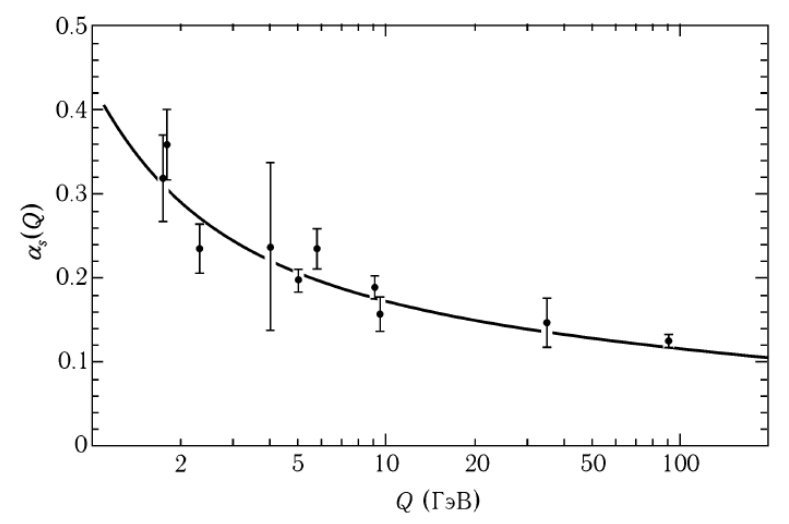
\includegraphics[width=0.8\textwidth]{13strong_coupling_constant_q.png}
        \caption[$\alpha_s$ dependence on $Q^2$]
        {Experimentally measured dependence of $\alpha_s$ on $Q$.
        The measured values are compared with the theoretical predictions of renormalised evolution with an initial value of $\alpha_s(m_z) = 0.117$ GeV.}
        % NOTE. Can't find a source :(.
        \label{fig::10.13::alpha_q_dependence}
    \end{figure}

